\documentclass[11pt]{article}
\usepackage[margin=0.66in]{geometry}
\usepackage{booktabs,enumitem,fancyhdr,graphicx,tabularx,titlesec}
\usepackage[table]{xcolor}
\usepackage[hidelinks]{hyperref}
\graphicspath{{docs/lessons/assets/}{../assets/}}
\hypersetup{pdftitle={ADK Lesson 045: Stationary Tabletop Balance Instrument},
 pdfauthor={Kevin Shanahan},
 pdfsubject={Atomic copied frames, explicit freeze authority, sensitivity, and deterministic replay},
 pdflang={en-US}}
\pagestyle{fancy}\fancyhf{}
\lhead{\textsc{ADK Lesson 045}}\rhead{Stationary Balance Instrument}
\cfoot{\thepage}\setlength{\headheight}{14pt}
\setlength{\parindent}{0pt}\setlength{\parskip}{4pt}
\setlist{nosep,leftmargin=1.45em}
\titleformat{\section}{\Large\bfseries}{\thesection}{0.5em}{}
\newcommand{\lessonbox}[1]{\begin{center}\fbox{\parbox{0.92\linewidth}{#1}}\end{center}}
\newcommand{\blankline}{\rule{0.86in}{0.4pt}}

\begin{document}
\begin{center}
 {\Huge\bfseries Stationary Balance Instrument}\\[3pt]
 {\Large Freeze one estimate; keep live evidence moving}\\[7pt]
 \fbox{\textbf{E0 SYNTHETIC REPLAY --- NO POWERED INERTIAL MODULE CLAIM}}
\end{center}
\begin{tabularx}{\linewidth}{@{}>{\bfseries}l X >{\bfseries}l X@{}}
Lesson & 045 --- project & Time & 120--180 minutes\\
Prerequisites & Lessons 043--044 & Board & compile-only Mega replay\\
Evidence & named memory result cells & Boundary & no bus, pins, wiring, or endpoints\\
\end{tabularx}

\lessonbox{\textbf{Project boundary.} This is a stationary, hand-tilted
tabletop instrument built from copied synthetic values and pure presentation
intent. It is not a balancing controller, handheld tracker, navigation aid,
vehicle instrument, safety device, or powered sensor demonstration.}

\section{Compose one atomic frame}
One \texttt{BalanceInstrumentInput} carries a copied inertial observation,
joystick observation, freeze-button observation, frame time, and frame
sequence. The caller snapshots each producer once. The instrument validates
the complete frame before committing any state.

\begin{tabularx}{\linewidth}{@{}l X X@{}}
\toprule
Copied producer & Identity & Required checks\\
\midrule
inertial & source, time, sequence, configuration and calibration &
freshness contract, readiness, quality, saturation, status\\
joystick & time and sequence & axes in \( -1000\ldots1000 \) permille,
event agrees with signs, status\\
button & time and sequence & pressed/event tuple is self-consistent, status\\
frame & frame time and sequence & forward modular order, no future producer,
bounded input skew\\
\bottomrule
\end{tabularx}

An exact delta-zero replay is idempotent. A changed field at the same identity
is malformed. A later frame may reuse the same immutable inertial sample, but
the instrument recomputes its age, freshness quality, sequence gap, and
derived status at the new frame time. It never fabricates a new sample.

\section{Follow live and frozen evidence}
\begin{center}
% ADK visual: pencil
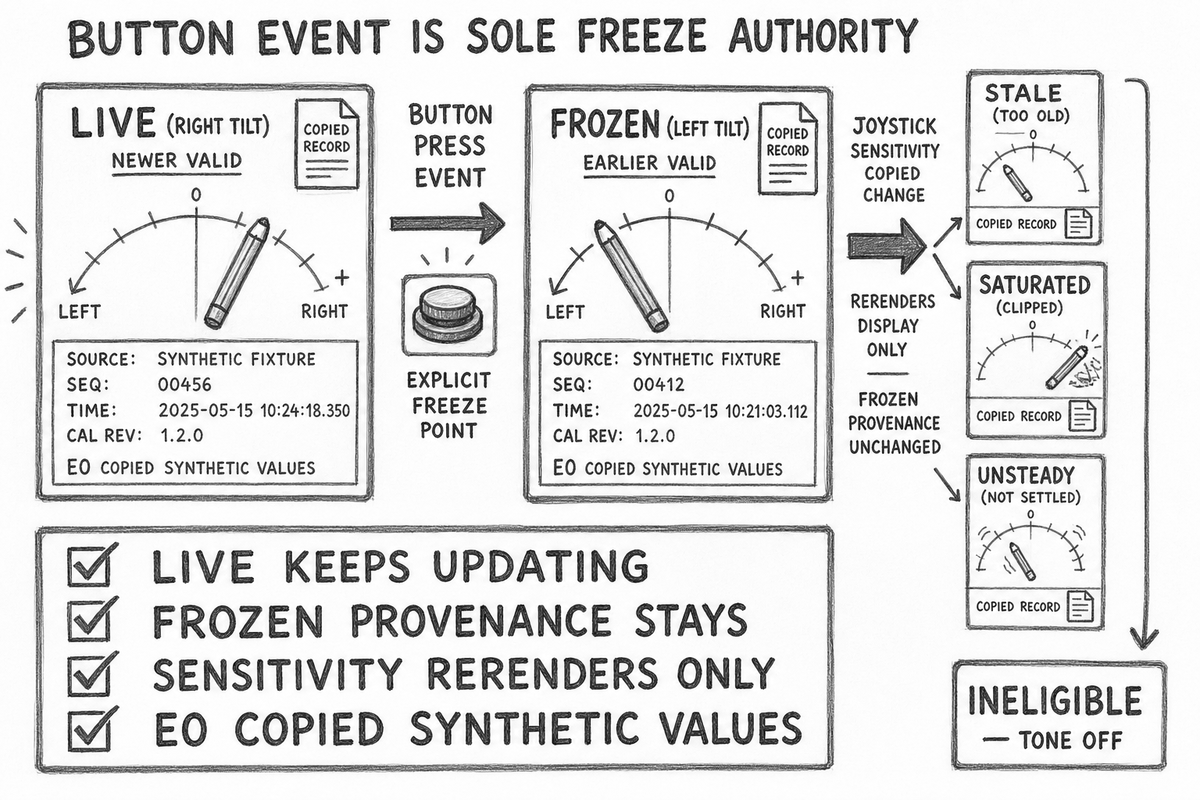
\includegraphics[width=0.96\linewidth,height=0.29\textheight,
 keepaspectratio]{045-live-frozen-pencil.png}

\small\textit{Alternative text: a pencil comparison shows current copied
inertial evidence feeding a live orientation while a button press copies the
current eligible estimate into a separate frozen evidence card. Later live
tilt and age continue changing beside the retained frozen comparison.}
\end{center}

Only a valid \texttt{pressEvent} is freeze authority. Tilt, sensitivity input,
a held button, and a replayed press cannot freeze. A valid press uses the
current frame's prepared estimate, not the previous snapshot. A second valid
press unfreezes. An invalid current estimate can never become frozen.

\begin{tabularx}{\linewidth}{@{}l X X@{}}
\toprule
Step & Predict & Observe in named result cells\\
\midrule
level frame & \texttt{Live} and eligible level estimate & live evidence available;
frozen unavailable\\
press with right tilt & \texttt{Frozen} & frozen evidence equals this frame's
right estimate\\
later forward tilt & frozen comparison remains right & live evidence changes
to forward\\
sensitivity increase & frozen estimate identity stays fixed & frozen
presentation is re-rendered at new sensitivity\\
unfreeze press & \texttt{Live} & current live evidence selects presentation\\
\bottomrule
\end{tabularx}

\section{Trace the state machine}
\begin{center}
% ADK visual: pencil
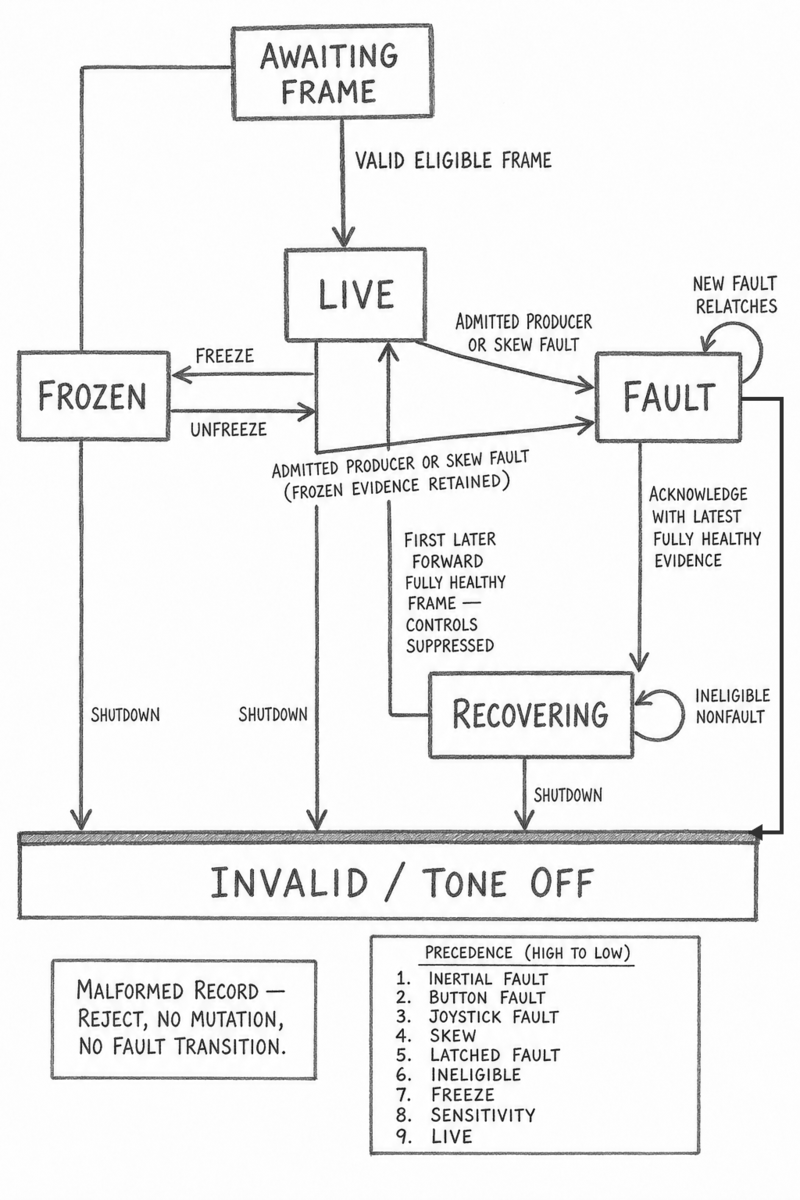
\includegraphics[width=0.96\linewidth,height=0.28\textheight,
 keepaspectratio]{045-state-flow-pencil.png}

\small\textit{Alternative text: a pencil state flow starts at AwaitingFrame,
moves between Live and Frozen only on eligible frames and explicit button
presses, latches Fault on an admitted producer or skew fault from either mode,
and requires acknowledgement plus a later healthy forward frame before
returning through Recovering. Malformed records reject without entering
Fault.}
\end{center}

\begin{tabularx}{\linewidth}{@{}l X@{}}
\toprule
Mode & Meaning\\
\midrule
\texttt{AwaitingFrame} & initialized, but no complete frame is accepted\\
\texttt{Live} & current eligible estimate selects presentation intent\\
\texttt{Frozen} & retained eligible estimate selects presentation while live
evidence still updates\\
\texttt{Fault} & a classified failure is latched; fault intent is tone-off\\
\texttt{Recovering} & acknowledgement succeeded; a later healthy forward frame
is still required\\
\bottomrule
\end{tabularx}

A healthy frame does not silently clear \texttt{Fault}.
\texttt{acknowledgeFault()} preserves evidence, sensitivity, replay identity,
and diagnostic epoch. The exact pre-ack replay cannot complete recovery.
A forward healthy frame does, while suppressing simultaneous freeze and
sensitivity events. Shutdown clears retained evidence and publishes the
configured invalid, tone-off intent.

\newpage
\section{Adjust sensitivity without changing evidence}
The joystick event changes only presentation sensitivity. Positive-only axes
mean \texttt{Increase}; negative-only axes mean \texttt{Decrease}; zero axes
mean \texttt{None}. Mixed positive and negative signs are an admitted
\texttt{Contradictory} no-op and make the complete frame not fully healthy.

\[
 s_{\mathrm{next}} =
 \mathrm{clamp}(s \mathbin{\pm} s_{\mathrm{step}},
 s_{\min},s_{\max})\quad\mathrm{permille}.
\]

\begin{tabularx}{\linewidth}{@{}X X X X@{}}
\toprule
current (permille) & event & step (permille) & next (permille)\\
\midrule
\rule{0pt}{16pt}\blankline & \blankline & \blankline & \blankline\\[9pt]
\blankline & \blankline & \blankline & \blankline\\[9pt]
\blankline & \blankline & \blankline & \blankline\\
\bottomrule
\end{tabularx}

Changing sensitivity never changes pitch, roll, source identity, timestamp,
sequence, or frozen provenance. It asks the Lesson 044 presentation policy to
render the selected estimate again. Every tone remains copied intent; this E0
lesson drives no sounder.

\section{Run the staged synthetic experiment}
\begin{center}
% ADK visual: pencil
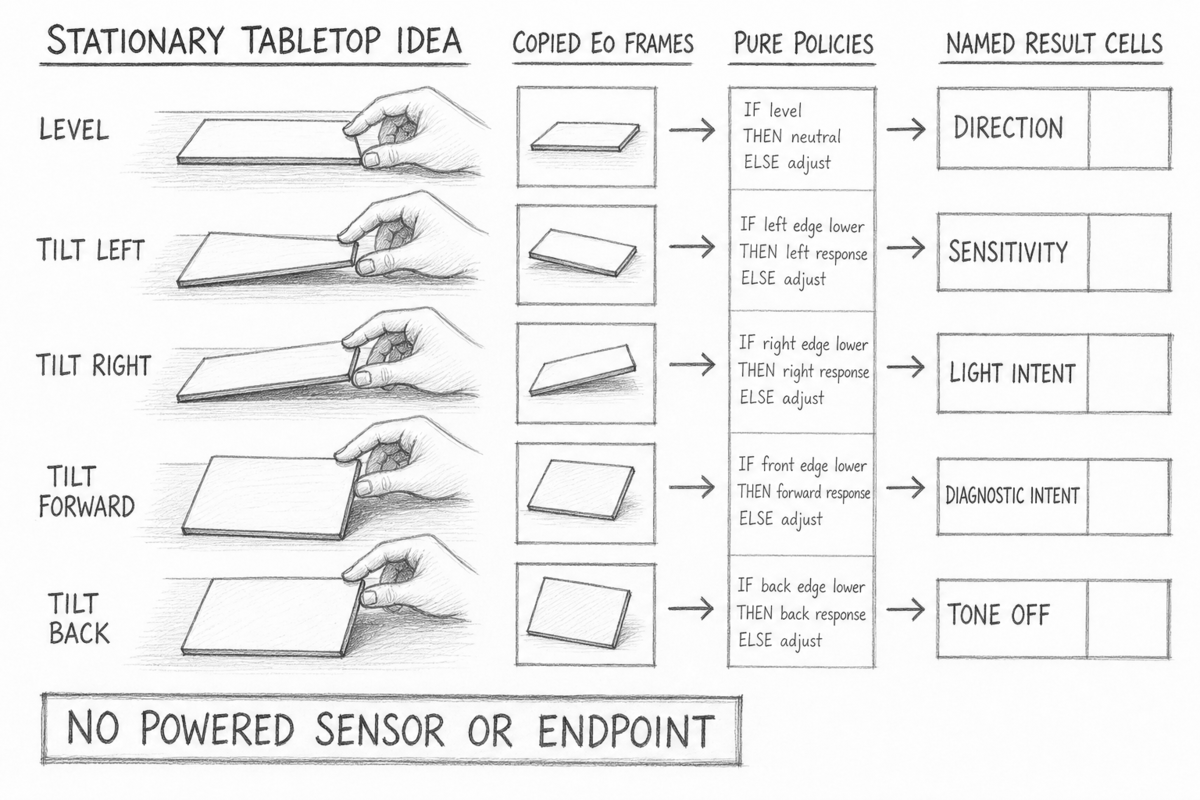
\includegraphics[width=0.97\linewidth,height=0.28\textheight,
 keepaspectratio]{045-tabletop-replay-pencil.png}

\small\textit{Alternative text: a pencil experiment strip stages startup,
level, cardinal tilts, sensitivity clamps, freeze, changed live tilt,
unfreeze, stale input, producer failure, acknowledgement, healthy recovery,
saturation, timestamp rollover, and shutdown as copied memory records.}
\end{center}

\begin{enumerate}
 \item Initialize. Predict \texttt{AwaitingFrame} with the configured
       tone-off presentation.
 \item Replay level and four cardinal tilts. Predict one complete live
       orientation and presentation record per accepted frame.
 \item Increase and decrease sensitivity through both clamps. Predict no
       wraparound and no change to measurement evidence.
 \item Freeze an eligible estimate, change the live tilt, and unfreeze.
       Predict distinct live and frozen evidence during comparison.
 \item Reuse an inertial sample in a later frame beyond its maximum age.
       Predict \texttt{Stale}, unavailable presentation eligibility, and
       tone-off intent without a fabricated producer event.
 \item Inject producer failure and acknowledge it. Predict \texttt{Fault},
       then \texttt{Recovering}; require a later healthy forward frame for
       \texttt{Live}.
 \item Replay saturation, timestamp rollover, exact duplicates, and shutdown.
       Predict stable identity, bounded intent, and no partial mutation.
\end{enumerate}

\section{Diagnose before interpreting}
\begin{tabularx}{\linewidth}{@{}>{\raggedright\arraybackslash}p{0.27\linewidth} l X@{}}
\toprule
Observation & Likely classification & Interpretation\\
\midrule
not ready or too old & \texttt{Stale} & accepted payload may remain, but it
is ineligible now\\
canonical axis limit reached & \texttt{Saturated} & do not interpret an
angle or enable tone\\
gravity/rate guard fails & \texttt{Unsteady} & stationary-orientation
assumption failed\\
source/configuration mismatch & invalid configuration & freshness or
provenance contract disagrees\\
future time or changed replay identity & malformed frame & reject without
mutating accepted state\\
producer age beyond input skew & \texttt{Fault} & commit canonical safe-state
evidence and advance replay identity\\
producer non-OK status & \texttt{Fault} & retain compact evidence and publish
fault-safe tone-off intent\\
\bottomrule
\end{tabularx}

\subsection*{Evidence worksheet}
\begin{tabularx}{\linewidth}{@{}X X X X@{}}
\toprule
frame time (ms) & sample time (ms) & age (ms) & quality/status\\
\midrule
\rule{0pt}{16pt}\blankline & \blankline & \blankline & \blankline\\[9pt]
\blankline & \blankline & \blankline & \blankline\\
\bottomrule
\end{tabularx}

\begin{tabularx}{\linewidth}{@{}X X X X@{}}
\toprule
frame sequence & sample sequence & live direction & frozen direction\\
\midrule
\rule{0pt}{16pt}\blankline & \blankline & \blankline & \blankline\\[9pt]
\blankline & \blankline & \blankline & \blankline\\
\bottomrule
\end{tabularx}

\section{Bound the E0 software resources}
AVR GCC 7.3 measurements use fixed storage and no heap, RTTI, exceptions,
virtual tables, Wire, or TWI. The application owns no timer or interrupt;
the linked Arduino startup/runtime still includes its ordinary timer-0
support.

\begin{tabularx}{\linewidth}{@{}X r X r@{}}
\toprule
Measured item & bytes & Measured item & bytes\\
\midrule
\texttt{BalanceInstrumentConfig} & 76 &
\texttt{BalanceInstrumentInput} & 101\\
caller replay storage & 102 &
\texttt{BalanceInstrumentOutput} & 119\\
inertial observation policy & 80 &
orientation policy & 38\\
presentation policy & 95 &
\texttt{BalanceInstrument} & 339\\
resident composition & 521 &
worst live composition & 741\\
\bottomrule
\end{tabularx}

The 339-byte instrument is below its revised 352-byte target and 384-byte hard
limit. Resident and worst-live results are below their 560/688-byte and
816/976-byte target/hard gates. The final expanded canonical sketch measures
26,398 bytes of flash (budget 28,672) and 1,898 bytes of static SRAM (budget
2,048).

The final no-LTO link measures 21,538 bytes of \texttt{.text}, 238 bytes of
\texttt{.data}, and 1,660 bytes of \texttt{.bss}; the latter two total the
1,898-byte static use. Compiler call-graph evidence bounds the foreground at
851 bytes. Conservatively adding the linked timer-0 interrupt's 15 bytes gives
866 bytes, leaving 5,428 bytes of SRAM---4,404 bytes above the 1,024-byte
margin gate. This is compiler and link evidence, not a runtime stack canary or
physical measurement. Runtime-canary evidence remains deferred to E1.

\section{Separate acquisition from safe state}
\textbf{Acquisition prediction.} A valid synthetic frame has recognized
source and status values, nonzero identities and freshness revision, bounded
producer skew, and self-consistent copied controls.

\textbf{Acquisition observation.} Inspect \texttt{acceptedFrameSequence},
\texttt{acceptedFrameAt}, producer statuses, compact live provenance, quality,
age, and availability in the host harness. Do not use Serial, a powered board,
or a hardware debugger.

\textbf{Acquisition interpretation.} Advancement means the complete copied
frame passed validation. It does not prove an inertial module, joystick,
button, clock, bus, or physical endpoint was acquired.

\textbf{Safe-state prediction.} Fault, ineligible quality, and shutdown each
publish a complete configured light record with tone disabled. Shutdown also
clears replay storage and retained measurement availability.

\textbf{Safe-state observation.} Inspect the copied mode, presentation,
tone-enabled field, live/frozen availability, and replay-storage availability
after each transition.

\textbf{Safe-state interpretation.} A canonical tone-off memory record proves
the pure policy result only. No physical LED, sounder, sensor pin, or supply
was made safe by this E0 replay.

\section{Open physical acceptance card}
\lessonbox{\textbf{Leave every field blank.} No powered inertial module,
joystick, button, RGB LED, diagnostic LED, sounder, bus, pin, resistor,
current, timing cadence, stack peak, or electrical shutdown has been observed
for this lesson. Compilation and synthetic replay are not bench acceptance.}

\begin{tabularx}{\linewidth}{@{}>{\bfseries}l X@{}}
Exact specimen and carrier markings & \rule{0pt}{16pt}\hrulefill\\[9pt]
Primary datasheet/register sources & \hrulefill\\[9pt]
Supply and logic-level qualification & \hrulefill\\[9pt]
Powered schematic review record & \hrulefill\\[9pt]
Measured rail/current and instruments & \hrulefill\\[9pt]
Physical observation and interpretation & \hrulefill\\[9pt]
Independent power-removal safe state & \hrulefill\\[9pt]
Reviewer, date, and acceptance record & \hrulefill\\
\end{tabularx}

A future E1 path requires exact, separately qualified hardware and an
electrically authoritative formal schematic. MPU-6050 qualification does not
qualify QMI8658, or vice versa. This E0 lesson publishes no wiring table,
address, register transaction, pin assignment, test point, or powered support
claim.

Any future platform must be lightweight, stable, entirely supported by the
table, and free of loose loads, sharp edges, pinch points, actuators, and
stored energy. The project never controls a launcher, vehicle, balancing
load, or safety mechanism.

\section{Software evidence and further work}
Deterministic tests cover lifecycle, atomic validation, semantic replay,
freeze authority, sensitivity clamps, freshness, precedence, recovery,
rollover, permutations, storage lifetime, and shutdown. The canonical Mega
sketch contains only copied fixture and result cells; compilation is packaging
evidence and the E0 sketch must not run on a powered board.

\begin{itemize}
 \item \href{https://github.com/spincyc/adk/blob/main/examples/Lesson045BalanceTableInstrument/Lesson045BalanceTableInstrument.ino}
       {Canonical compile-only Lesson 045 sketch}.
 \item \href{https://github.com/spincyc/adk/blob/main/tests/test_balance_table_instrument.cpp}
       {Deterministic balance-instrument tests}.
 \item \href{https://github.com/spincyc/adk/blob/main/src/balance_table_instrument.h}
       {Balance-instrument interface}.
 \item \href{https://github.com/spincyc/adk/blob/main/docs/design/LESSONS_043_045_BALANCE_TABLE_PLAN.md}
       {Lessons 043--045 design record}.
 \item \href{https://github.com/spincyc/adk/blob/main/docs/TESTING.md}
       {Deterministic testing contract}.
 \item \href{https://github.com/spincyc/adk/blob/main/docs/PDF_POLICY.md}
       {PDF visual policy}.
 \item \href{https://github.com/spincyc/adk/blob/main/docs/SAFETY_MODEL.md}
       {Safety model}.
\end{itemize}

This untagged print edition has a searchable HTML alternative.
It makes no PDF/UA or physical accessibility claim.
\end{document}
